\chapter{Design}
\label{ch:design}
WebGL promises a new generation of 3D web games.
However the problem of transporting the assets over the network in an acceptable timeframe is challenging.
One way of dealing with it is to use some of the procedural content generation techniques discussed in Chapter~\ref{ch:backgroundpcg}.
However, how to incorporate those techniques into a new technology such as WebGL is not obvious.

This chapter will present the design of a system which uses procedural content generation to generate the plans of buildings in WebGL.
The design presented is very general however, and can be used as a template for anyone incorporating any kind of procedural content generation into their projects on any platform.

\section{Design Goals}
\label{sec:designgoals}
Our main goals for this project were:
\begin{itemize}
    \item Scenes which resemble a current game
    \item Ability to assess performance relative to a non-procedural version
    \item Easy to edit design program
	\item Use a generic approach which can be applied on different platforms and with different procedural techniques
\end{itemize}

When it came to deciding on which texture effects would be implemented, perlin noise and bump mapping were chosen due to their wide use in games~\cite{web:perlingames}~\cite{kilgard2000practical}.
At all aspects of this project, real-time interactive frame rates and reasonable loading times were seen as being necessary, as these are necessary for modern games.

\subsection{Ability to Assess Performance}
This goal led me to the separation of the project into two applications:
\begin{itemize}
	\item One which allows the user to design the plan and generate geometry to be output to a file
	\item One which displays the geometry using WebGL and can either procedurally generate the content on the fly or can read in the assets from files.
\end{itemize}

Two different frameworks were chosen, based on their suitability for the task.
Processing~\cite{web:processing} was chosen as the language for the design program.
Processing is written in the Java programming language, which the author was already very familiar with.
Processing has a lot of built in features for displaying and drawing 2D patterns, and it was thus ideal for displaying the plan generated to the user.
It also easily allows the programmer to write information to files.

GwtGL~\cite{web:gwtgl} was chosen as the framework for the WebGL application itself.
It has the advantage that it is written in the Java programming language, compiled to javascript using the Google Web Toolkit~\cite{web:gwt} compiler.
This made code reuse possible between the main WebGL application and the design application.
In particular, the geometry generation stages were identical in code.
The author would encourage anyone doing similar work to consider these frameworks.
In particular processing is a very flexible framework and is very performant.

\subsection{Intuitive Design Program}
The design program was designed so that the output could be configured by a small number of input variables.
The program is such that it should be editable by novice programmers such as artists, etc.
The input variables which can be modified are very centred around the apperance of the output.
For example the width and height of rooms in the plans are two of the parameters to the application.
Other parameters include the height on the y-axis of the projected plan in 3D.
Another parameter is the maximum number of rooms in the plan in the x and y axes.
With the modification of these parameters, it is possible to generate a variety of plans.
A few example designs are shown in Figure~\ref{fig:designapp}.

\begin{figure}
  \centering
  \subcaptionbox{Input: xRoom=3, yRoom=4, nRooms=4}{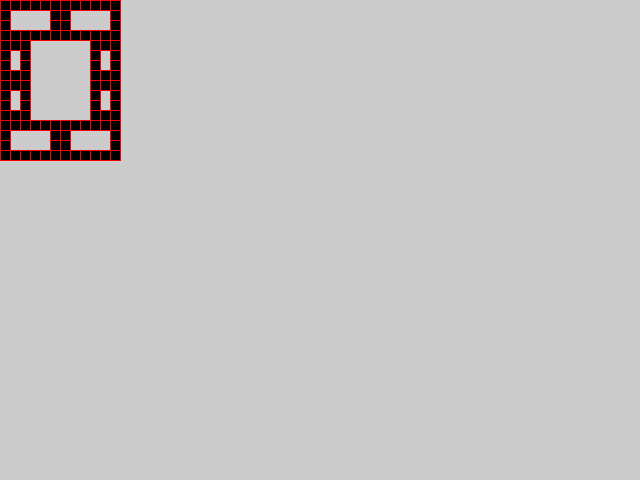
\includegraphics[width=0.4\textwidth]{images/plan/screen0}}
  \subcaptionbox{Input: xRoom=3, yRoom=4, nRooms=5}{
\includegraphics[width=0.4\textwidth]{images/plan/screen1}}
  \subcaptionbox{Input: xRoom=3, yRoom=5, nRooms=9}{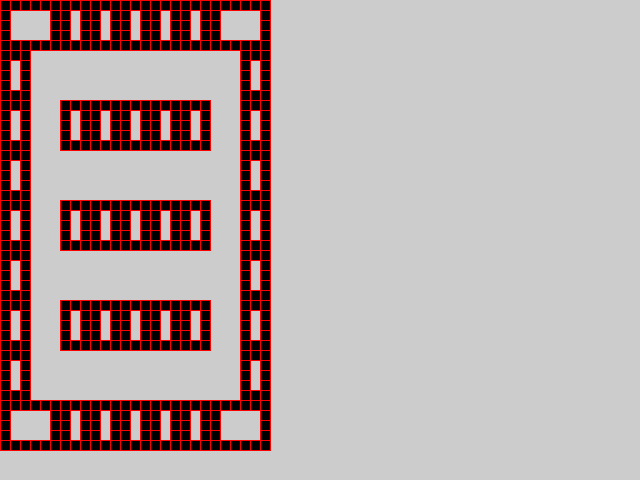
\includegraphics[width=0.4\textwidth]{images/plan/screen2}}
  \subcaptionbox{Input: xRoom=5, yRoom=3, nRooms=11}{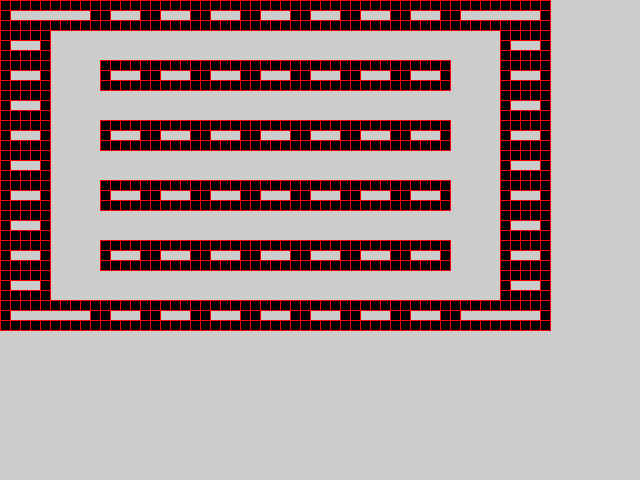
\includegraphics[width=0.4\textwidth]{images/plan/screen3}}
  \caption{Different Plans generated using the design program}
  \label{fig:designapp}
\end{figure}

\section{General Architecture}
The architecture of the system is divided into two distinct applications for the reasons described in Section~\ref{sec:designgoals}.
The general architecture is depicted in Figure~\ref{fig:sysarch}.
The architecture shows which parts of the system are shared between the 2 applications, and which parts are distinct.

This architecture should hold for any project which uses procedural content generation, though the specific methods of how the geometry is generated will likely change from project to project.
This project is an implementation of this generic architecture and should be seen as a proof-of-concept that this architecture works in practice.
The architecture's design is based on that presented by Greuter et. al in 2003~\cite{greuter2003undiscovered}, with the main exception being that our architecture also includes texture generation explictly as part of the architecture and a design program.

The input parameters are as follows:
\begin{itemize}
	\item xRoom : The size of each room along the X-Axis
	\item yRoom : The size of each room along the Y-Axis
	\item nRooms : The number of rooms to generate in the resulting plan on each axis
\end{itemize}
These input parameters affect the way the resultant plan appears.

\begin{figure}
  \centering
  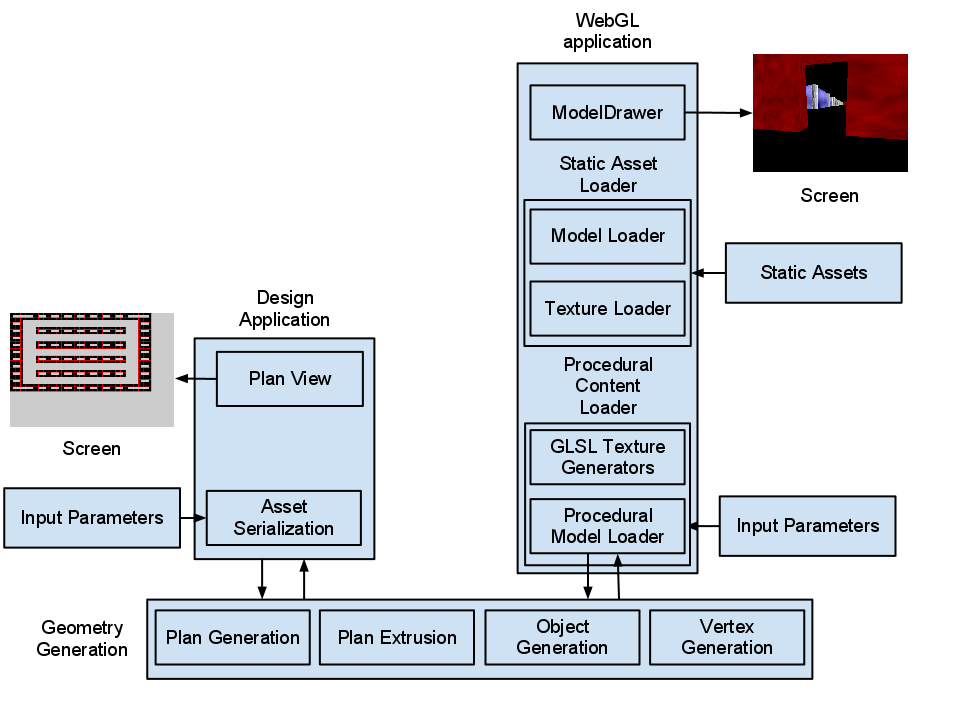
\includegraphics[width=\textwidth]{images/gwtprocArchitecture}
  \caption{System Architecture}
  \label{fig:sysarch}
\end{figure}

We will now focus our attention on both parts of this application in turn.

\subsection{Geometry Generation}
\label{sec:desgeomgen}
The phases involved in the geometry generation process are quite general in nature.
The plan generation phase is influenced by the input parameters.
It generates rooms in a grid-like fashion, and places other objects such as pillars in their locations.
The Plan Extrusion process involves creating objects from the rooms generated during plan generation.
Object generation creates objects based on certain parameters.
For instance the pillars are generated to defined level by progressive refinement.
Vertex Generation involves creating a collection of vertex objects which have enough information to render.

\subsection{Design Application}
The design application's purpose is to take a number of parameters as input and to output geometry in the form of files which can be read by the WebGL application.
The vertices for the rooms and other objects are retrieved from the Geometry Generation process.
The rooms are then drawn to the screen by the Plan View.
This gives the user an impression of what the resulting geometry will look like.
The Asset Serialization stage uses the Geometry Generation process described in Section~\ref{sec:desgeomgen} and converts the resultant vertices to Strings.
It then writes these strings to different output files, depending on the model being generated. 
These files can then be parsed and loaded by the WebGL Application.

\subsection{WebGL Application}
The WebGL application can either read in static assets from files or it can procedurally generate the assets, using the common Geometry Generation stages.
A flag is set in the WebGL application to indicate which version has been chosen.
If the static assets version of the application has been chosen, no procedural content generation is done - the assets are read in from files.
For textures this means loading in image files and for models it means reading files of text representing the information for the vertices.

When procedural content generation has been chosen it uses common Geometry Generation phases to get the vertex information for the models.
The procedural model loader is influenced by the input parameters and in this way models with varying complexity and size can be generated.

%\section{Experiment Design}
%Experiments were designed to be reproduceable and to be fair to both versions of the prototype.
